\documentclass[12pt]{article}

\pagestyle{empty}
\setlength{\topmargin}{0in}
\setlength{\headheight}{0in}
\setlength{\topsep}{0in}
\setlength{\textheight}{9in}
\setlength{\oddsidemargin}{0in}
\setlength{\evensidemargin}{0in}
\setlength{\textwidth}{6.5in}

\usepackage{palatino, graphicx}

\newcommand{\real}{{\bf R}}
\newcommand{\maple}[1]{\medskip\hspace{.25in}\begin{tt} > {\bf #1}
  \end{tt}\medskip} 
\newcommand{\col}[3]{\left[\begin{array}{c} #1 \\ #2 \\ #3\end{array}
  \right]}
%\newcommand{\mmatrix}{4}{\left[ \begin{array}{cc} #1 & #2 \\
%#3 & #4 \end{array}\right]}
\newcommand{\woodyn}{Wooody}
\newcommand{\woody}{Wooody\ }      


\begin{document}

\noindent
{\bf Mathematics 227} \\ 
{\bf Lab 2, Due: October 17, 2018}

\bigskip

\noindent
{\bf Instructions:} The exercises here should be completed in groups
of 2 or 3 students with one write-up submitted from each group.

\medskip
In this lab, we'll see how computer
animators use matrix transformations to tell stories.  In fact, if you
saw {\em Incredibles 2} last summer, you were seeing some very elegant
applications of linear algebra.

Now, let me introduce you to \woodyn, the lovable star of the animated
kids' film {\em Toy Tale} due out this holiday season.  

\medskip
\begin{center}
  \includegraphics{woody.eps}
\end{center}
\medskip

The computer animators who made {\em Toy Tale} assembled the film
frame by frame.  To make us think that \woody is moving, they make
changes in \woodyn's position from one frame to the next.  This is
where linear algebra is useful.  (Actually, \woody really lives in a
three-dimensional world and each part of his body may be moving in
different ways so the situation is a little more complicated but
hopefully you will get the idea.)

If you go to {\tt http://gvsu.edu/s/0Jb}, you will find a figure that
can make \woody move.  On the left, you see a picture of \woodyn,
while on the right you will see a picture of him after a matrix
transformation has been applied.

Here is the function we will consider;  it is
not quite as simple as what we have seen in class:
\begin{eqnarray*}
x_r & = & ax_l + by_l + c \\
y_r & = & dx_l + ey_l + f
\end{eqnarray*}
The six sliders along the top of the diagram represent the quantities
$$\begin{array}{ccc}
a & b & c \\
d & e & f.
\end{array}
$$

\bigskip
\begin{enumerate}
\item  Using homogeneous coordinates, we represent this change as
  $$
  \left[\begin{array}{c} x_r \\ y_r \\ 1 \end{array}\right] = 
  \left[\begin{array}{ccc}
      a & b & c \\
      d & e & f \\
      0 & 0 & 1
    \end{array}\right]
  \col{x_l}{y_l}{1}.$$

  Compute this matrix product and verify that it produces the
  appropriate expressions for $x_r$ and $y_r$.

  \vspace*{1.5in}
  
\item  Press the {\bf Reset} button if you have modified
  \woodyn.  As shown above, \woody is waving with his left hand.  In
  the first scene of the movie, \woody comes on screen and waves with
  his right hand.  What is the matrix transformation that has been
  applied?  

  \includegraphics{woody1.eps}

  \bigskip
\item  Next, \woody begins his morning callesthenics and performs
  a cartwheel.  
% The film's producer wants to remind you that the linear
%   transformation defined by the matrix
%   $$
%   \left[\begin{array}{ccc}
%       \cos \theta & -\sin \theta & 0 \\
%       \sin \theta & \cos \theta & 0 \\
%       0 & 0 & 1
%     \end{array}\right]
%   $$
%   has the geometric effect of rotating vectors in the plane
%   counterclockwise by an angle of $\theta$.
  Write the transformations which produce the following sequence of
  pictures. 

  \begin{tabular}{cc}
    \includegraphics{woody20.eps} ~~~ & ~~~
    \includegraphics{woody21.eps} \\
    \includegraphics{woody22.eps} ~~~ & ~~~
    \includegraphics{woody23.eps} 
  \end{tabular}
  
\newpage
\item  At this point in the story, \woody suddenly remembers a
  long-ago love and the camera moves in for a close up.
  \begin{center}
    \includegraphics{woody40.eps} ~~~
    \includegraphics{woody41.eps} ~~~
    \includegraphics{woody42.eps} 
  \end{center}
  
  There are two ways to do this, but one is easy after a little
  thought.  The first two frames are rather straightforward.  The
  third is a little tricky but the diagram gives you another tool to
  help.  Once you have the diagram configured in some way you like,
  you may press the button {\bf Apply}, the image on the left is set
  to that on the right and the transformation reset to the identity.
  You may then operate on the new figure from scratch.
  (Mathematically, you are composing two functions.)

  Explain a simple way to make the sequence of frames above.  

  \vspace*{2in}

  Determine the function that takes our original picture of \woody into
  the final close up?

  \vspace*{1in}

  \newpage
  \item  \woody decides to go out for a walk.  In the morning sun,
    he casts a shadow that looks like this:
    
    \begin{center}
      \includegraphics{woody50.eps}
    \end{center}

    Find a matrix transformation which creates the
    shadow.  You might remember how we have found the matrix
    representing a matrix transformation by looking at the image of
    the standard basis vectors.

    \vspace*{1in}

    As the sun comes up, his shadow get shorter.

    \begin{center}
      \includegraphics{woody51.eps} ~~~
      \includegraphics{woody52.eps}
    \end{center}

    Explain what matrix transformations achieve this and how you found
    them.  (Think about composing transformations again.)

    \vspace*{1.15in}

    % \item[6.]  In a scene edited from the final version to maintain a
    %   G rating, \woody decides to unwind at Studio $(1, -2)$.

    %   \begin{center}
    %     \includegraphics[100 400 200 500]{woody60.eps}
    %   \end{center}
      
    %   What is the linear transformation here?

    %   \vspace*{1in}

    %   The camera moves in for a close up and \woody's head starts to
    %   spin.  

    %   \begin{center}
    %     \includegraphics[100 400 200 500]{woody61.eps} ~~~
    %     \includegraphics[100 400 200 500]{woody62.eps}  \\
    %     \medskip
    %     \includegraphics[100 400 200 500]{woody63.eps} ~~~
    %     \includegraphics[100 400 200 500]{woody64.eps} 
    %   \end{center}

    %   Explain how to do this.  Think geometrically and try to break
    %   the operation down into smaller, more manageable pieces.

    %   \vspace*{2in}

    \item Write an ending to our heart-felt story and describe how to
      illustrate it.


\end{enumerate}






\end{document}